%%%% CAPÍTULO 3 - MATERIAL E MÉTODOS (PODE SER OUTRO TÍTULO DE ACORDO COM O TRABALHO REALIZADO)

\chapter{Metodologia}\label{cap:materialemetodos}

O projeto foi estruturado em duas etapas principais: o desenvolvimento da
infraestrutura de \textit{hardware} e a criação do \textit{software}.
Além da criação do protótipo físico, foi elaborado um código com o 
objetivo de alcançar desempenho otimizado, atendendo a todos os 
requisitos do projeto. Isso incluiu desde a fase inicial de inicialização 
até a implementação de uma interface gráfica para os usuários, a entrada 
de dados, o reconhecimento facial, o cadastro e exclusão de usuários, 
por fim, o módulo de acionamento.

O fluxograma apresentado na \autoref{fig:fluxoprog} oferece uma visão
simplificada do funcionamento do \textit{software} do projeto. O sistema
de controle de acesso por biometria facial opera em dois ciclos principais:
o primeiro é dedicado à autenticação do usuário, enquanto o segundo é responsável
pelo cadastro de usuários. Além disso, há um ciclo obrigatório com um
temporizador em execução em segundo plano. Esse ciclo é ativado
automaticamente sempre que um dos ciclos principais é iniciado, com o intuito
de encerrar quaisquer atividades pendentes e prevenir possíveis \textit{loops}
dentro do sistema.

\begin{figure}[h!]
    \centering
    \caption{Fluxograma do \textit{firmware}}
    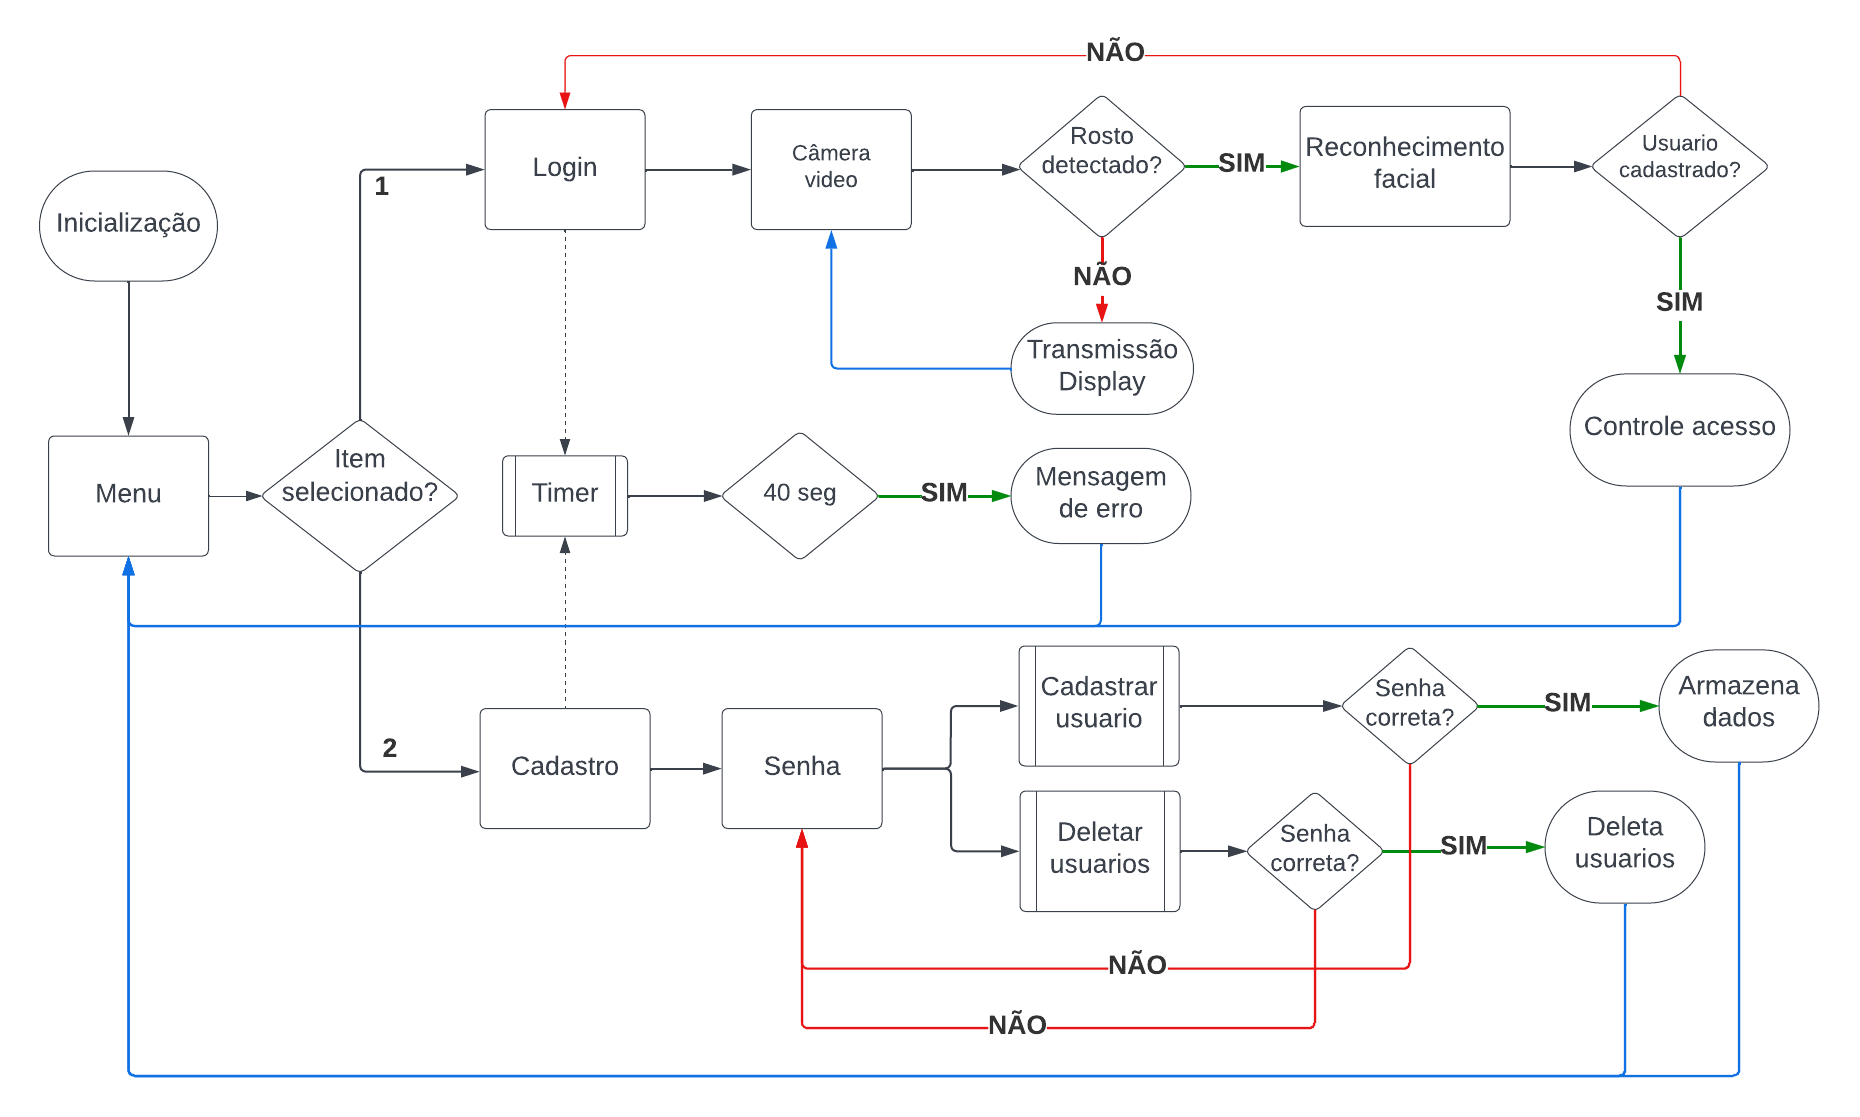
\includegraphics[scale=0.25]{figuras/fluxo_app.png}
    \fonte{}%% Fonte
    \label{fig:fluxoprog}
    \centering
\end{figure}

Para a execução desse programa, é necessário o uso de um \textit{hardware}
capaz de processá-lo. Portanto, a primeira etapa do projeto foi dedicada à
construção do protótipo físico. E com o intuito de facilitar a compreensão desta
parte do projeto, foi criado o diagrama apresentado na \autoref{fig:fluxohard}.
Conforme evidenciado, o ESP32-CAM é o módulo central, encarregado do
processamento de dados e da coordenação das informações aos demais módulos.
Para melhorar a interação com os usuários, é adicionado o módulo com botões e
uma interface gráfica (\textit{display}). Por fim, o módulo relé é
responsável pelo controle de acesso, podendo acionar diferentes tipos de
fechaduras elétricas.

\begin{figure}[h!]
    \centering
    \caption{Diagrama de blocos do \textit{hardware}}
    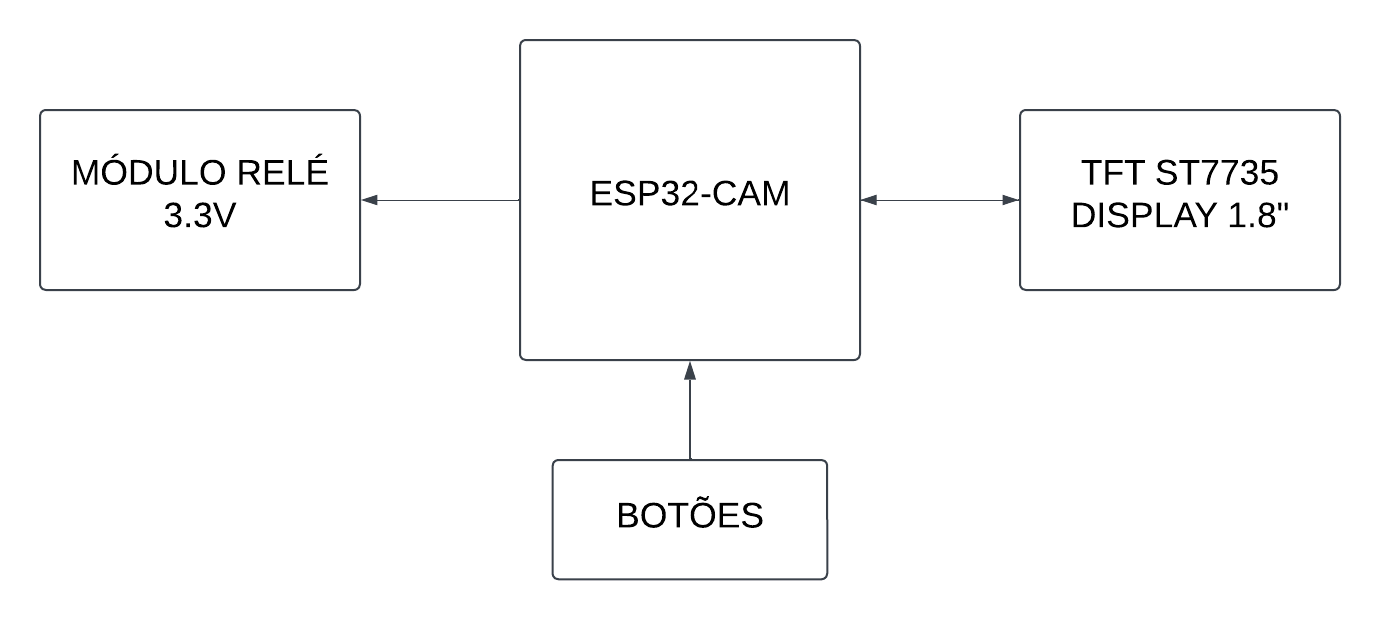
\includegraphics[scale=0.22]{figuras/diagrama_hardware.png}
    \fonte{}%% Fonte
    \label{fig:fluxohard}
    \centering
\end{figure}

Como um dos objetivos do projeto é o desenvolvimento de um protótipo de
baixo custo, a versão selecionada para essa finalidade é o ESP32-CAM,
que se destaca por integrar um \textit{chip} ESP32, uma câmera, uma
entrada para cartão SD e LED de alto brilho.

\section{Microcontrolador ESP32-CAM}\label{sec:materiais}

O ESP32-CAM (conforme ilustrado na \autoref{fig:espcam}) é um
microcontrolador de alto desempenho, desenvolvido pela empresa
\textit{Espressif Systems}® e que se destaca por sua acessibilidade.
Embora compacto, é uma escolha ideal para este projeto devido à sua
rica variedade de recursos e vantagens. Ele apresenta uma câmera
integrada à placa, um processador dual-core de 32 bits capaz de
executar tarefas em tempo real e disponibiliza 16 pinos de
Entrada/Saída (E/S).

Neste projeto, o ESP32-CAM desempenhou um papel central, sendo
responsável pelo processamento de dados, análise das informações
e controle dos demais componentes de \textit{hardware}. Isso incluiu
o gerenciamento de dispositivos adicionais e a coordenação das funções
necessárias para a aplicação proposta.

\begin{figure}[h!]
    \centering
    \caption{ESP32-CAM}
    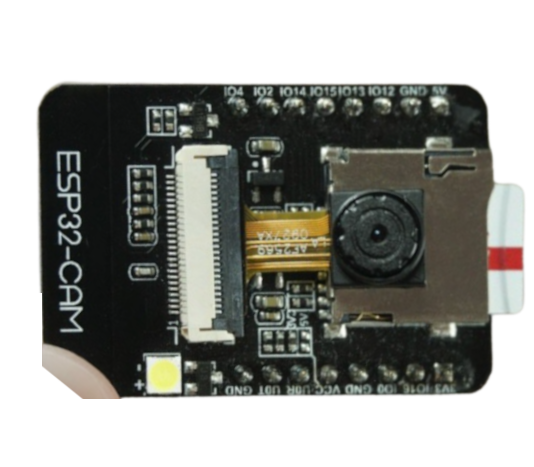
\includegraphics[scale=0.25]{figuras/esp32cam.png}
    \legend{Fonte: Adaptado de \citeonline{espcamimg}.}
    \label{fig:espcam}
    \centering
\end{figure}

\subsection{Pinos de Entrada/Saída (E/S)}\label{sec:gpio}

Os 16 pinos de Entrada/Saída (E/S) do ESP32-CAM (\autoref{fig:esp32pin})
desempenham um papel crucial na versatilidade
e funcionalidade deste microcontrolador.
Esses pinos oferecem uma interface flexível para conectar o
ESP32-CAM a uma ampla variedade de dispositivos e periféricos
externos, permitindo que ele interaja com o ambiente e execute
tarefas específicas de acordo com as necessidades do projeto.

\begin{figure}[h!]
    \centering
    \caption{GPIO disponíveis do ESP32-CAM}
    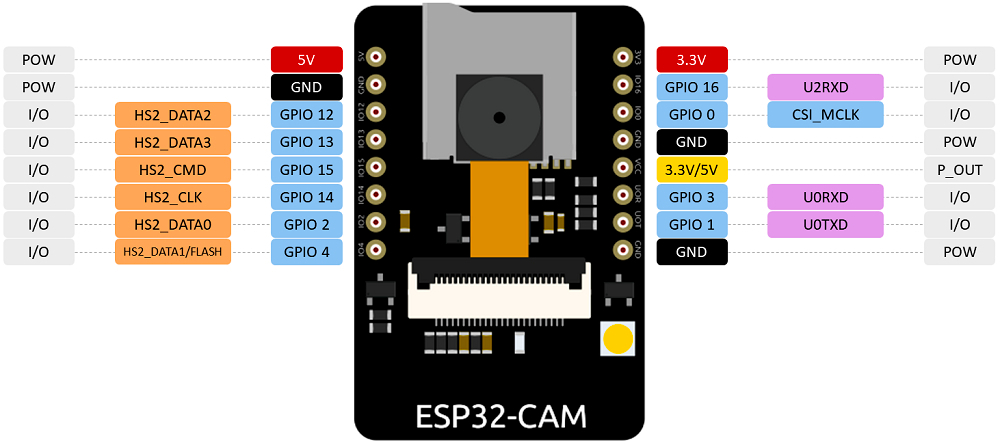
\includegraphics[scale=0.28]{figuras/esp32pin.jpg}
    \legend{Fonte: Adaptado de \citeonline{esp32pin}.}
    \label{fig:esp32pin}
    \centering
\end{figure}

Esses pinos são fundamentais para a comunicação com sensores, atuadores,
dispositivos de armazenamento, \textit{displays} e muitos outros componentes
eletrônicos, tornando o ESP32-CAM
adequado para inúmeras aplicações, desde sistemas de
segurança e monitoramento, até projetos de automação residencial.

No quadro a seguir (\autoref{quad:quadro1}), são detalhadas as funcionalidades dos 16 pinos 
de Entrada/Saída (E/S) disponíveis no ESP32-CAM. O entendimento destes pinos, possibilita 
aos desenvolvedores a flexibilidade de personalizar e expandir suas 
aplicações de acordo com suas necessidades específicas.

\begin{tabframed}[htb]
    \caption{Portas de Entrada/Saída ESP32-CAM}
    \label{quad:quadro1}
    \begin{tabular}{|l|l|}
        \hline
        \textbf{Pinos} & \textbf{Descrição}                                                                          \\ \hline
        5V             & Pino de entrada para alimentação do circuito do ESP32.                                      \\ \hline
        3GND           & 3 pinos de aterramento, usado para referência de potencial zero.                          \\ \hline
        GPIO12         & Pino de propósito geral.                                                                    \\ \hline
        GPIO13         & Pino de propósito geral.                                                                    \\ \hline
        GPIO15         & Pino de propósito geral.                                                                    \\ \hline
        GPIO14         & Pino de propósito geral.                                                                    \\ \hline
        GPIO2          & Pino de propósito geral.                                                                    \\ \hline
        GPIO4          & Pino de propósito geral e pode ser utilizado para acionar o Flash do ESP32.                 \\ \hline
        3.3V           & Pino de fornecimento de energia de 3,3V.                                                    \\ \hline
        GPIO16         & Este pino sempre fica em nível lógico alto e é utilizado para alimentar o circuto de PSRAM. \\ \hline
        GPIO0          & Pino de propósito geral, entretanto este pino é responsável pelo clock da câmera.           \\ \hline
        3.3V/5V        & Pode fornecer energia de 3,3V ou 5V para outros dispositivos.                               \\ \hline
        GPIO3          & Pino de entrada de dados UART (RX) para comunicação serial.                                 \\ \hline
        GPIO1          & Pino de saída de dados UART (TX) para comunicação serial.                                   \\ \hline
    \end{tabular}
    \fonte{}%% Fonte
\end{tabframed}

\section{Interface gráfica}\label{sec:interface}

O \textit{Display} LCD TFT (\textit{Thin-Film Transistor}) de 1.8 polegadas, 
com resolução de 128x160 \textit{pixels}
e \textit{driver} ST7735 (\autoref{fig:tft7735}) é um componente popular 
utilizado em uma variedade de aplicações eletrônicas, devido à sua 
capacidade de fornecer uma interface visual clara e interativa. 
Esse tipo de \textit{display} é frequentemente empregado em projetos que requerem 
a exibição de informações, gráficos e interação direta com o usuário.

Neste contexto, o uso deste \textit{display} no projeto tem o propósito de aprimorar 
a experiência do usuário, fornecendo uma representação visual clara da 
aplicação. Além disso, sua biblioteca de fácil utilização simplifica o 
processo de desenvolvimento do projeto, tornando-o mais acessível e eficaz.

\begin{figure}[h!]
    \centering
    \caption{\textit{Display} LCD TFT 1.8"}
    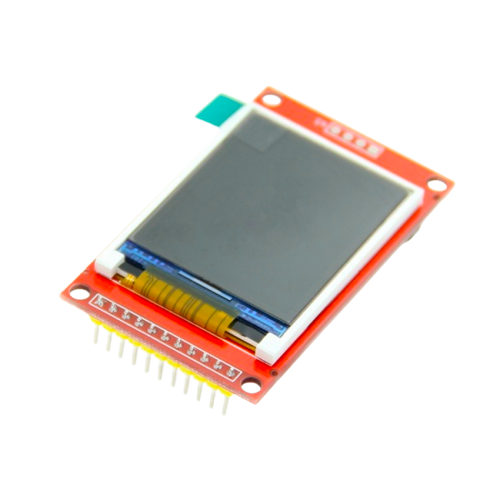
\includegraphics[scale=0.4]{figuras/tftst7735.png}
    \legend{Fonte: Adaptado de \citeonline{tft7735img}.}
    \label{fig:tft7735}
    \centering
\end{figure}

\section{Módulo de acionamento}\label{sec:acionamento}

Um módulo relé, como apresentado na \autoref{fig:rele}, é um componente 
eletrônico amplamente utilizado em projetos que envolvem controle 
e automação de dispositivos elétricos. Ele desempenha 
um papel essencial ao permitir o controle de circuitos 
de alta potência por meio de sinais de baixa potência.

\begin{figure}[h!]
    \centering
    \caption{Módulo Relé}
    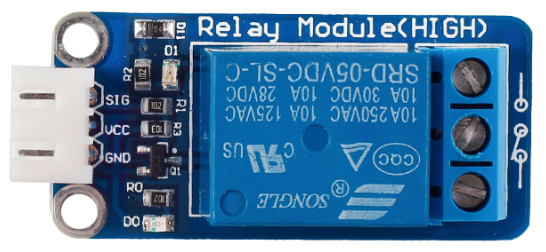
\includegraphics[scale=0.8]{figuras/rele.png}
    \fonte{\citeonline{releimg}}%% Fonte \legend{Fonte: Adaptado de \citeonline{releimg}.}
    \label{fig:rele}
    \centering
\end{figure}

Quando se trata de fechaduras eletrônicas, os módulos relé desempenham um 
papel crucial, facilitando o funcionamento e a segurança do sistema de 
controle de acesso. Geralmente, essas fechaduras 
incluem um mecanismo de trinco que pode ser controlado eletronicamente. 
O módulo relé é utilizado para controlar a ativação e desativação 
desse mecanismo, quando um usuário autorizado fornece uma credencial 
válida (como uma senha, cartão RFID ou impressão digital), o sistema 
eletrônico de controle gera um sinal de baixa potência para acionar 
o módulo relé. O relé fecha seu contato, permitindo a passagem de 
energia para o mecanismo de destravamento da fechadura, liberando 
assim o acesso.

\section{Desenvolvimento do \textit{software}}\label{sec:software}

Para o desenvolvimento do \textit{software}, foi essencial escolher uma plataforma 
de desenvolvimento capaz de programar e gravar códigos nos microcontroladores 
ESP32. Duas opções amplamente conhecidas são o Arduino IDE e o PlatformIO. 
Além disso, o desenvolvimento exigiu um estudo aprofundado das 
bibliotecas disponíveis para atender aos requisitos do projeto, 
tais como o reconhecimento facial, transmissão em tempo real de 
imagens em um \textit{display} LCD, implementação de um \textit{timer} e a manipulação 
dos dados de entrada e saída.

\subsection{PlatformIO}\label{sec:platformio}

A plataforma escolhida para esse projeto foi o PlatformIO, 
que é uma ferramenta indispensável para quem trabalha com dispositivos 
microcontrolados, como o ESP32. Projetado para simplificar o processo 
de desenvolvimento e programação de microcontroladores, o PlatformIO 
oferece uma ampla gama de recursos e uma abordagem unificada que 
facilita o trabalho com diferentes plataformas de \textit{hardware} e 
ambientes de desenvolvimento.

Quando se trata do ESP32, o PlatformIO desempenha 
um papel crucial, permitindo que desenvolvedores e entusiastas de 
eletrônica programem e depurem suas aplicações de maneira eficiente.
O PlatformIO é projetado para funcionar com diversos editores de 
código populares, como \textit{Visual Studio Code} (VSCode), Atom e CLion. 
Isso permite que os desenvolvedores escolham a IDE que melhor 
se adapte às suas preferências.

Por fim, outros dois outros pontos fortes da ferramenta PlatformIO podem 
ser citados: a plataforma possui um gerenciador de bibliotecas embutido que facilita a 
pesquisa, instalação e atualização de bibliotecas de código-fonte 
aberto. Isso é particularmente útil para reutilizar código 
existente e acelerar o desenvolvimento, como também sua 
simplificação no processo de compilação e carregamento de 
código para o \textit{hardware} de destino. 

\subsection{Biblioteca ESP-DL}\label{sec:formatacaoTexto}

Para identificação de rostos e reconhecimento facial, foram utilizados 
os recursos disponíveis da biblioteca ESP-DL.

O ESP-DL é uma biblioteca de alto desempenho dedicada ao ESP32, ESP32-S2,
ESP32-S3 e ESP32-C3, projetada para recursos de aprendizagem profunda.

O \citeonline{espdl} disponibiliza APIs para tarefas como inferência 
de redes neurais (NN), processamento de imagens, operações matemáticas 
e inclui alguns modelos de aprendizado profundo. Com essa biblioteca, 
os desenvolvedores podem aproveitar os SoCs (System-on-Chip) da 
\textit{Espressif} de maneira simples e ágil para a implementação 
de uma ampla variedade de aplicações.

Dentre os recursos disponíveis do ESP-DL, se encontra o 
ESP-Face, componente que fornece funções de detecção e 
reconhecimento facial e também operações de rede neural. 
O método \textit{face detect} utiliza o modelo MTMN (\textit{Multi-Task 
Mobile Nets}).

No contexto do reconhecimento facial, uma vez que um rosto 
humano tenha sido detectado por meio do procedimento 
mencionado anteriormente, é possível realizar uma verificação 
comparando-o com os rostos previamente cadastrados. 
A entrada para esse processo é a imagem original juntamente 
com os resultados obtidos na etapa de detecção facial.

O método de reconhecimento facial, denominado \textit{recognize face}  
faz uso do modelo FRMN (\textit{Face Recognition Memory Network}), que 
também se baseia na arquitetura móvel \textit{MobileNetV2} e emprega o 
algoritmo \textit{ArcFace}.

\subsection{Fluxo de telas}\label{sec:telas}

Os recursos gráficos fornecidos pelo \textit{display} LCD desempenham um papel 
fundamental na usabilidade da aplicação. Nesse contexto, a elaboração 
do fluxo de telas se torna essencial para proporcionar aos usuários 
uma experiência eficiente. Todos os fluxos foram planejados e 
projetados com o objetivo de guiar o usuário por meio 
de diferentes interações e funcionalidades.

O primeiro conjunto de telas (\autoref{fig:fluxoinicial}), referente à 
inicialização dos recursos utilizados no programa do protótipo, 
abrange o momento em que a câmera, os sensores e o SPIFFS 
(Sistema de Arquivos Flash de Interface Serial Periférica) 
são ativados. Além disso, a lista de usuários cadastrados é 
inicializada antes de exibir a tela de menu.

\begin{figure}[h!]
    \centering
    \caption{Telas de inicialização}
    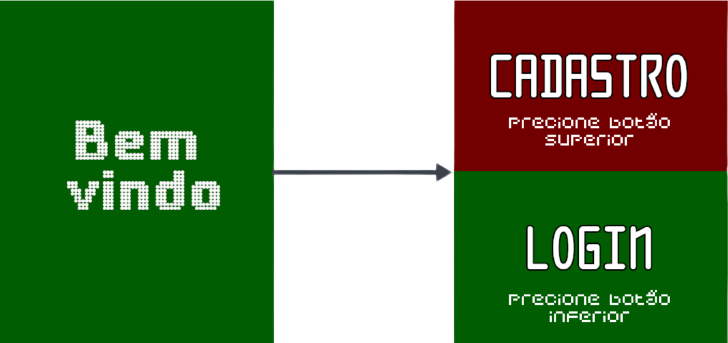
\includegraphics[scale=0.25]{figuras/fluxo_inicial.png}
    \fonte{}%% Fonte
    \label{fig:fluxoinicial}
    \centering
\end{figure}

Ao chegar no menu e selecionar a opção de login, o usuário inicia o 
fluxo de telas de login. Inicialmente, é exibida uma mensagem de 
orientação para enquadrar o rosto dentro do campo de visão da câmera. 
Se o usuário estiver cadastrado, uma mensagem de sucesso é exibida 
e em seguida, o módulo do relé é acionado. Caso contrário, o \textit{timer} 
é executado em segundo plano e quando o tempo se esgota, uma mensagem 
de erro é exibida, como representado na \autoref{fig:fluxologin}.

\begin{figure}[h!]
    \centering
    \caption{Fluxo de telas do login}
    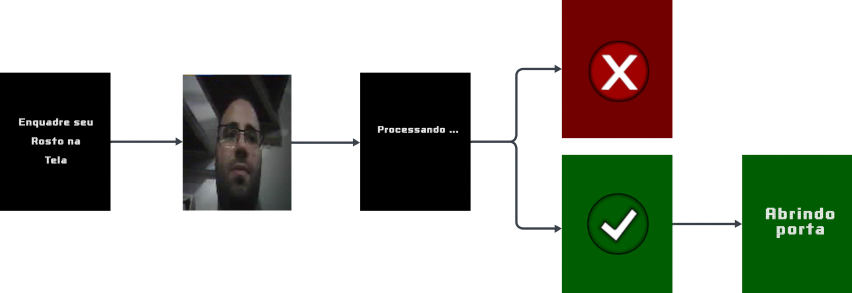
\includegraphics[scale=2.1]{figuras/fluxo_login.png}
    \fonte{}%% Fonte
    \label{fig:fluxologin}
    \centering
\end{figure}

No entanto, se o usuário escolher a opção de cadastro no menu, 
ele deverá seguir o fluxo descrito na \autoref{fig:fluxocadastro}. 
Na primeira etapa, é solicitado ao usuário para digitar a senha. 
Se a senha estiver correta, uma mensagem de ''senha correta'' é 
exibida e o processo de identificação e reconhecimento facial 
é iniciado. Se tudo ocorrer conforme o esperado, os dados são 
armazenados na memória RAM ou na memória flash. Caso contrário, 
o usuário visualizará uma mensagem de erro.

\begin{figure}[h!]
    \centering
    \caption{Fluxo de telas do cadastro}
    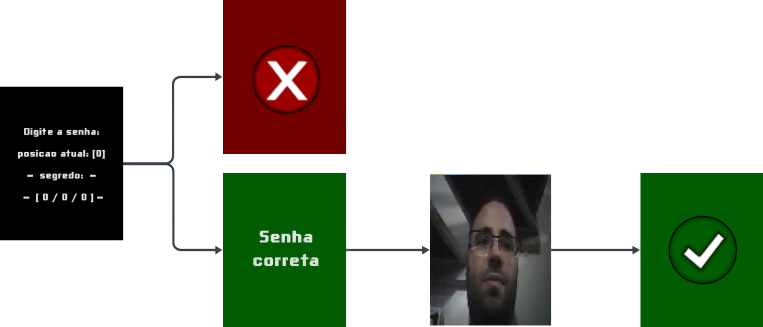
\includegraphics[scale=2]{figuras/fluxo_cadastro.png}
    \fonte{}%% Fonte
    \label{fig:fluxocadastro}
    \centering
\end{figure}


Por fim, o último fluxo principal é o processo de exclusão 
de usuários (\autoref{fig:fluxosenha}), que se assemelha 
ao fluxo de cadastro. Como observado, em ambos 
os casos, a primeira tela solicita a inserção 
da senha e o usuário tem aproximadamente 40 segundos 
para descobrir ou digitar a senha correta. Durante esse processo, 
podem ser exibidas mensagens de erro ou sucesso. Se tudo ocorrer 
conforme o esperado, a mensagem ''usuários deletados'' é exibida.

\begin{figure}[h!]
    \centering
    \caption{Fluxo de telas para deletar usuário}
    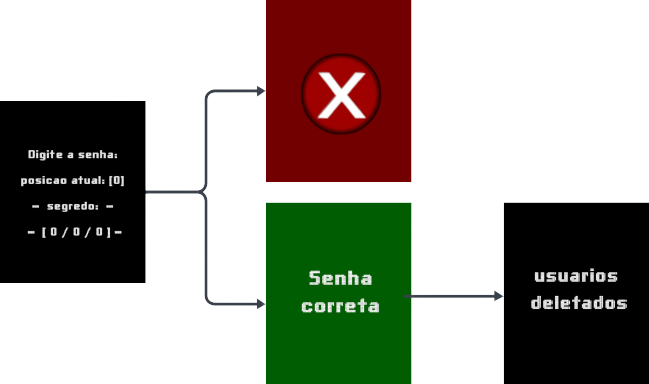
\includegraphics[scale=1.8]{figuras/fluxo_deletar_usuario.png}
    \fonte{}%% Fonte
    \label{fig:fluxosenha}
    \centering
\end{figure}

\subsection{Gravação do código}\label{sec:gravador}

Para a gravação do código no ESP32-CAM, foi essencial o uso do módulo 
adaptador ESP32-CAM MB (conforme representado na 
\autoref{fig:adaptadoresp32}). Este módulo desempenhou um papel importante, 
estabelecendo uma conexão entre o ESP32-CAM e um computador por meio 
do cabo USB.

Para desenvolvimento do protótipo, elaborou-se um diagrama elétrico 
detalhado, conforme ilustrado na \autoref{fig:circuito}. Este diagrama 
foi construído com base em um circuito previamente testado e montado em 
uma placa de prototipagem (''\textit{protoboard}''). A escolha dos conectores do 
tipo borne KRE para as conexões de entrada e saída se justifica pela 
praticidade e segurança que oferecem, devido ao seu encaixe lateral que 
simplifica a conexão com os componentes eletrônicos.

\begin{figure}[h!]
    \centering
    \caption{Módulo Adaptador ESP32-CAM MB}
    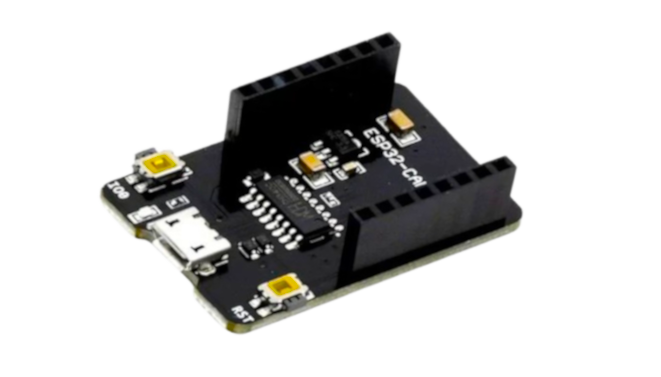
\includegraphics[scale=0.25]{figuras/adaptador_esp32cam.png}
    \legend{Fonte: Adaptado de \citeonline{adaptadoresp32}.}
    \label{fig:adaptadoresp32}
    \centering
\end{figure}

\section{Desenvolvimento do protótipo}\label{sec:prototipo}

Para desenvolvimento do protótipo, foi fundamental criar um diagrama 
elétrico detalhado para guiar a montagem do circuito. O diagrama 
apresentado na \autoref{fig:circuito}, foi elaborado com base no 
circuito pré-testado e montado em uma placa de prototipagem (''\textit{protoboard}'').

\begin{figure}[h!]
    \centering
    \caption{Diagrama elétrico do protótipo}
    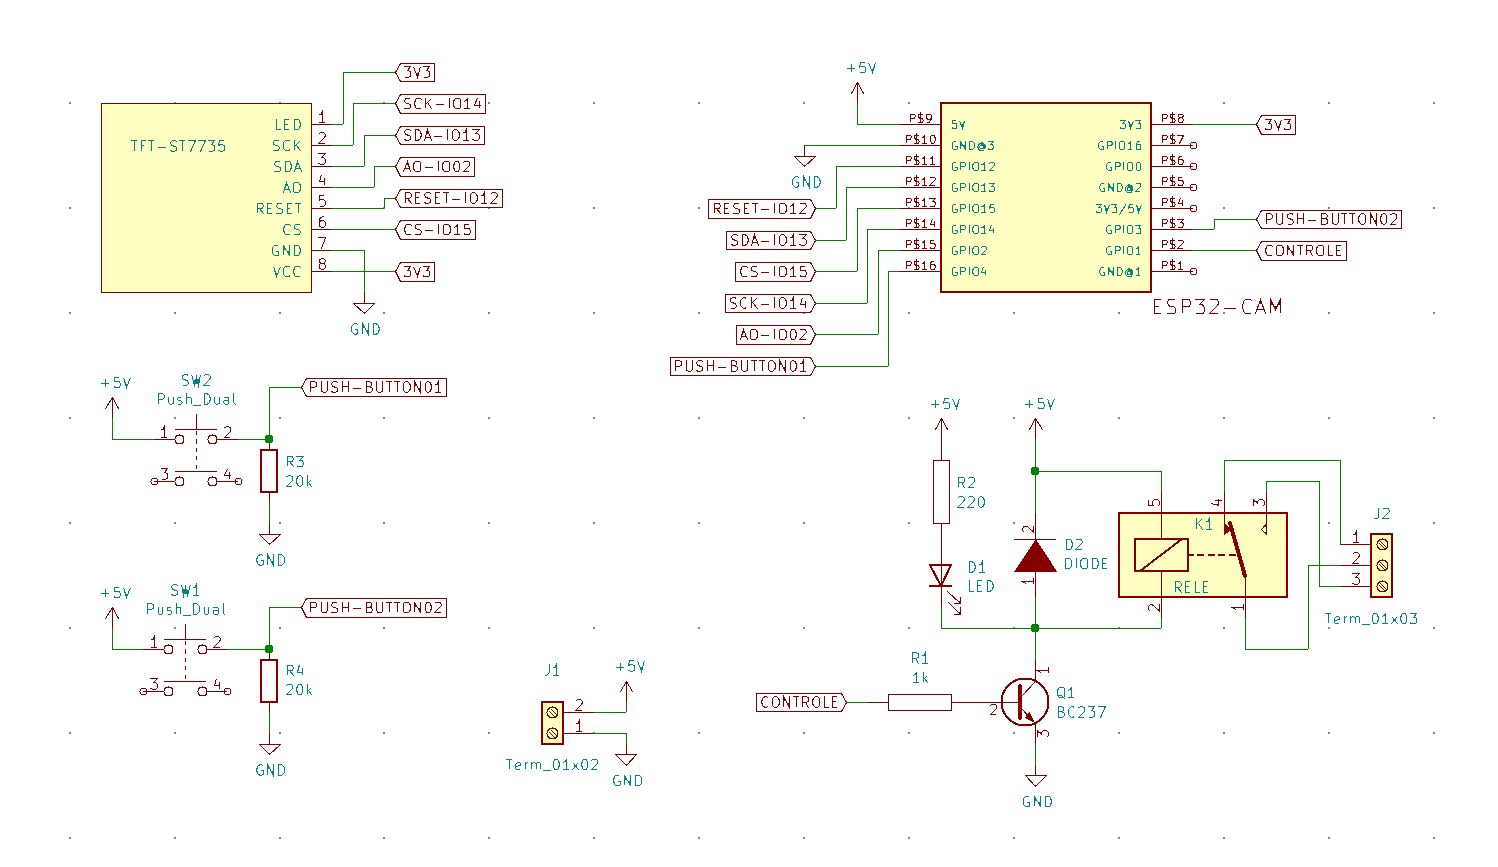
\includegraphics[scale=0.3]{figuras/circuito_completo.png}
    \fonte{}%% Fonte
    \label{fig:circuito}
    \centering
\end{figure}

O diagrama elétrico do protótipo divide o circuito em quatro blocos 
principais: o ESP32-CAM, o TFT ST7735, o módulo de relé e o módulo 
de botões (\textit{push button}). O bloco principal, que é o ESP32-CAM, 
possui 16 pinos de entrada/saída (GPIOs), como representado na 
\autoref{fig:diagramaesp} e desempenha o papel de controle e 
coordenação do sistema como um todo. Dos 16 pinos disponíveis, 
7 são dedicados ao \textit{display} TFT (GPIOs 2, 12, 13, 14 e 15), 2 são 
reservados para os botões (GPIOs 4 e 3) e 1 pino é utilizado 
como saída para controlar o módulo do relé (GPIO 1).

Importante mencionar que algumas GPIOs têm funções específicas. 
Por exemplo, a GPIO 16 permanece em nível lógico alto e é utilizada 
para habilitar a memória PSRAM. Além disso, a GPIO 0 é designada como 
\textit{clock} da câmera e não pode ser realocada para outras finalidades, 
uma vez que isso afetaria o funcionamento adequado da captura de 
imagens. Essas atribuições de GPIOs foram cuidadosamente 
planejadas para garantir o correto funcionamento de 
cada componente do protótipo. 

\begin{figure}[h!]
    \centering
    \caption{Diagrama elétrico do ESP32-CAM}
    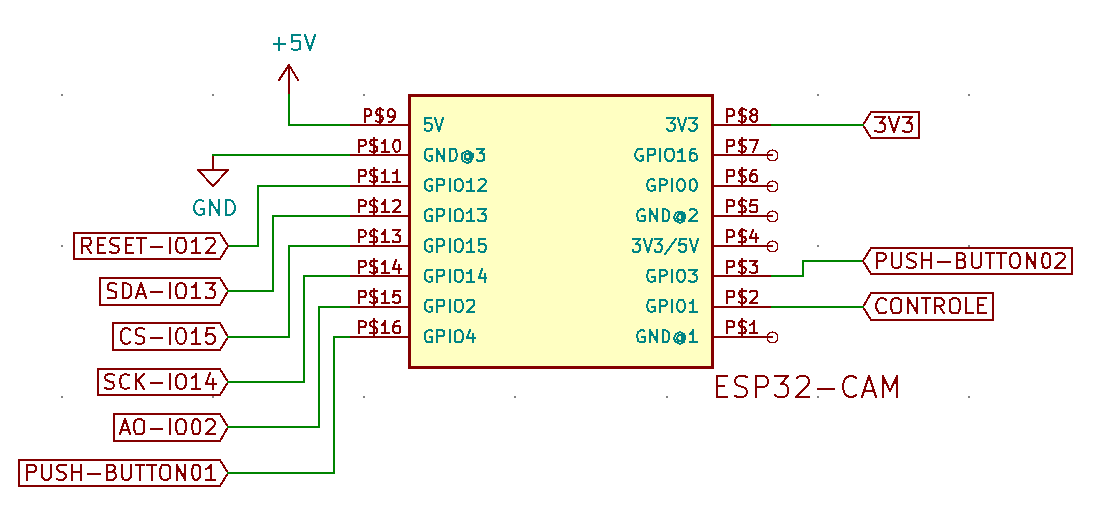
\includegraphics[scale=0.3]{figuras/modulo_esp.png}
    \fonte{}%% Fonte
    \label{fig:diagramaesp}
    \centering
\end{figure}

O segundo bloco corresponde ao controlador ST7735 (\autoref{fig:diagramatft}), 
um componente projetado para o gerenciamento de \textit{displays} TFT de tamanho 
reduzido e com capacidade de exibir cores. A principal função desse 
controlador é administrar a apresentação de informações na tela, 
permitindo a criação de gráficos e a exibição de texto colorido.

A tela em si é composta por uma matriz de \textit{pixels} coloridos, em que 
cada \textit{pixel} é formado por subpixels nas cores vermelha, verde e azul 
(RGB), possibilitando a exibição de uma vasta gama de cores. Os pinos 
SCK (\textit{Serial Clock}), SDA e CS (\textit{Chip Select}) são utilizados para a 
comunicação serial com o microcontrolador. Por sua vez, o pino de 
\textit{reset} é designado para reiniciar o \textit{display} em caso de falhas ou erros.

Adicionalmente, o pino A0 desempenha um papel fundamental ao indicar 
se os dados transmitidos se referem a comandos de controle (estado \textit{LOW}) 
ou a dados de \textit{pixel} (estado \textit{HIGH}), desempenhando um papel crucial no 
funcionamento adequado do controlador ST7735.

\begin{figure}[h!]
    \centering
    \caption{Diagrama elétrico do \textit{Display} TFT}
    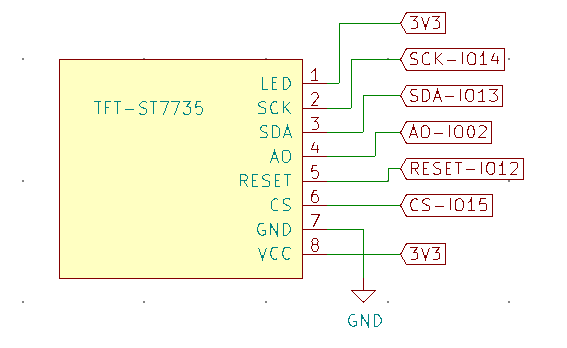
\includegraphics[scale=0.36]{figuras/modulo_tft.png}
    \fonte{}%% Fonte
    \label{fig:diagramatft}
    \centering
\end{figure}

O bloco que compreende os botões desempenha um papel fundamental na 
interatividade do projeto, pois permite a seleção de itens no menu 
e a inserção dos valores da senha. 

A estrutura dos botões é 
ilustrada no circuito apresentado na \autoref{fig:diagramabotoes}, e 
cada botão é capaz de enviar um sinal de nível lógico baixo quando não 
pressionado e de nível lógico alto quando acionado, transmitindo esses 
sinais ao microcontrolador.

Devido a mudança de estado do botões ao alterar o sinal elétrico conforme 
são pressionados ou soltos, permite ao microcontrolador reconhecer as ações 
do usuário, possibilitando a navegação no aplicativo de forma eficiente 
e prática. Isso torna esses componentes essenciais para a interatividade 
do protótipo e contribuem significativamente para a experiência do usuário.

\begin{figure}[h!]
    \centering
    \caption{Diagrama elétrico dos botões}
    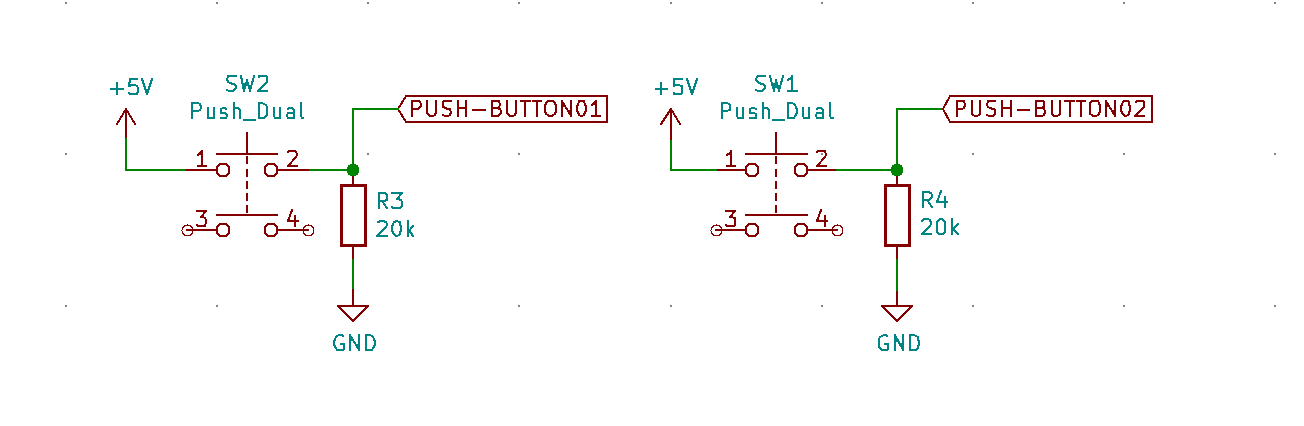
\includegraphics[scale=0.25]{figuras/modulo_push.png}
    \fonte{}%% Fonte
    \label{fig:diagramabotoes}
    \centering
\end{figure}

O relé é um dispositivo eletromecânico amplamente utilizado para o controle 
de circuitos elétricos, permitindo a comutação (abertura ou fechamento) 
por meio de um sinal elétrico aplicado à sua bobina.

O módulo de relé, conforme apresentado na (\autoref{fig:diagramarele}), 
consiste em um circuito que viabiliza que um microcontrolador 
envie um sinal de baixa potência para a base de um transistor. A conexão do 
coletor do transistor à bobina do relé viabiliza o seu acionamento 
quando o transistor entra em estado de saturação. Isso, por sua vez, permite que o ESP32 
controle dispositivos de alta potência por meio de sinais de baixa potência. 
Um elemento crucial nesse circuito é o diodo em paralelo ao relé, 
que também é conhecido como diodo de roda livre.

O diodo de roda livre desempenha um papel essencial na proteção do 
circuito contra picos de tensão e corrente gerados quando a bobina 
do relé é desativada. Esse fenômeno ocorre devido à interrupção 
abrupta da corrente que fluía através da bobina, criando uma sobretensão 
reversa que poderia potencialmente danificar os componentes do circuito. 
O diodo age como um caminho de baixa resistência para a corrente, 
permitindo um caminho controlado para a dissipação da energia excedente, 
evitando danos aos componentes sensíveis do circuito. Portanto, o diodo 
de roda livre é crucial para garantir a integridade e a confiabilidade 
do sistema elétrico.

\begin{figure}[h!]
    \centering
    \caption{Diagrama elétrico do módulo relé}
    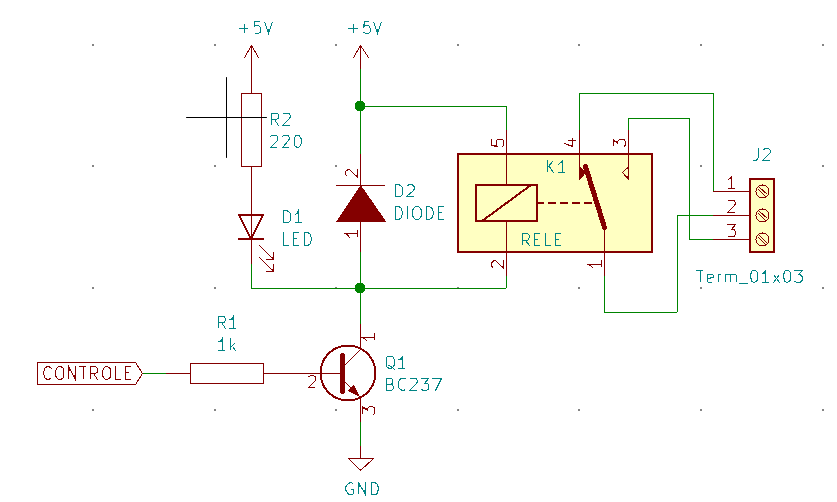
\includegraphics[scale=0.2]{figuras/modulo_rele_esquema.png}
    \fonte{}%% Fonte
    \label{fig:diagramarele}
    \centering
\end{figure}

Com base no esquema elétrico e na necessidade de criar um protótipo 
compacto e eficiente, o projeto da PCB (\textit{Printed Circuit Board} ou 
Placa de Circuito Impresso) foi concebido com o objetivo de otimizar 
o aproveitamento de espaço, como pode ser observado na \autoref{fig:placapcb}. 
Nessa placa, os componentes estão dispostos de forma organizada, 
seguindo uma lógica de uso e, ao mesmo tempo, minimizando o espaço 
ocupado para garantir uma solução compacta e funcional. A disposição 
estratégica dos componentes na PCB é crucial para a eficiência e o 
desempenho do protótipo.

\begin{figure}[h!]
    \centering
    \caption{Projeto da placa de circuito impresso do protótipo}
    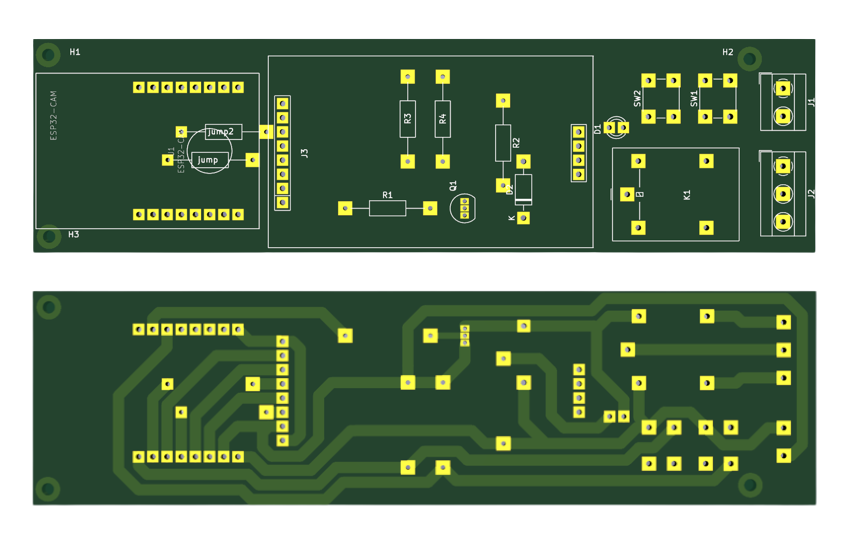
\includegraphics[scale=0.25]{figuras/placa_pcb.png}
    \fonte{}%% Fonte
    \label{fig:placapcb}
    \centering
\end{figure}

Após a conclusão do projeto da PCB, procedeu-se à fabricação da placa e 
à integração dos componentes eletrônicos. Como ilustrado na \autoref{fig:placamanufaturada}, 
foram adicionados os componentes de acordo com o projeto. Uma escolha 
estratégica foi a inclusão de barras de pinos fêmea no lugar dos 
conectores do ESP32-CAM e do \textit{Display} TFT. Essa decisão visou 
possibilitar a remoção e substituição desses componentes com 
facilidade. Esse recurso é especialmente útil para o ESP32, 
permitindo a conexão a um gravador de código externo sempre 
que necessário, proporcionando maior flexibilidade e 
versatilidade ao protótipo.

\begin{figure}[h!]
    \centering
    \caption{Placa manufaturada}
    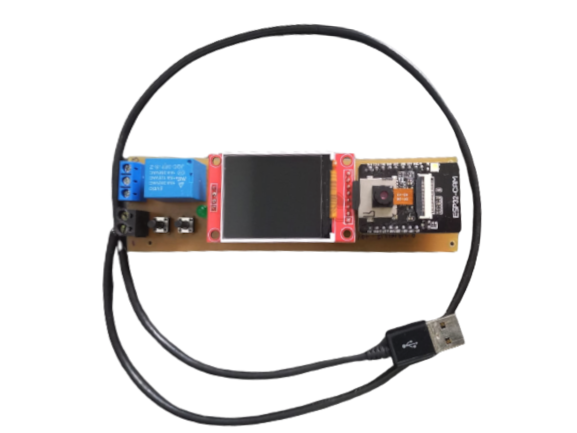
\includegraphics[scale=0.35]{figuras/placa_montada.png}
    \fonte{}%% Fonte
    \label{fig:placamanufaturada}
    \centering
\end{figure}

Como parte final do processo, uma caixa foi projetada e fabricada para cumprir 
dois propósitos essenciais: proteger o circuito eletrônico e oferecer um 
acabamento esteticamente agradável para o usuário. A caixa, como ilustrada 
na \autoref{fig:placamontada}, foi dimensionada a partir das dimensões da placa 
já confeccionada. A modelagem 3D foi realizada para que a caixa pudesse 
ser impressa em 3D e posteriormente acoplada à placa. Esse invólucro 
não apenas protege o protótipo, mas também contribui para uma 
apresentação mais profissional e amigável ao usuário, resultando em 
uma experiência mais agradável de uso.

\begin{figure}[h!]
    \centering
    \caption{Placa montada}
    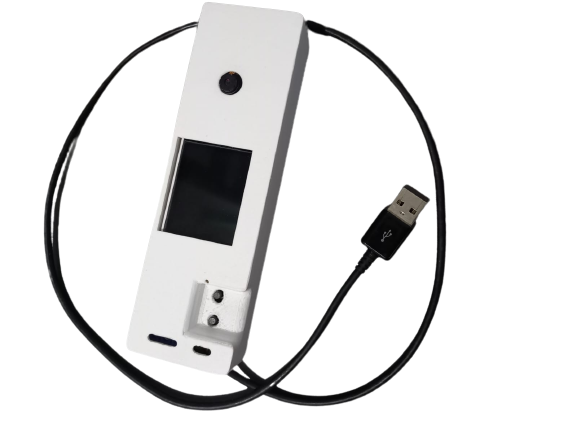
\includegraphics[scale=0.3]{placa_case.png}
    \fonte{}%% Fonte
    \label{fig:placamontada}
    \centering
\end{figure}